% TEMPLATE for Usenix papers, specifically to meet requirements of
%  USENIX '05
% originally a template for producing IEEE-format articles using LaTeX.
%   written by Matthew Ward, CS Department, Worcester Polytechnic Institute.
% adapted by David Beazley for his excellent SWIG paper in Proceedings,
%   Tcl 96
% turned into a smartass generic template by De Clarke, with thanks to
%   both the above pioneers
% use at your own risk.  Complaints to /dev/null.
% make it two column with no page numbering, default is 10 point

% Munged by Fred Douglis <douglis@research.att.com> 10/97 to separate
% the .sty file from the LaTeX source template, so that people can
% more easily include the .sty file into an existing document.  Also
% changed to more closely follow the style guidelines as represented
% by the Word sample file. 

% Note that since 2010, USENIX does not require endnotes. If you want
% foot of page notes, don't include the endnotes package in the 
% usepackage command, below.

% This version uses the latex2e styles, not the very ancient 2.09 stuff.
\documentclass[letterpaper,twocolumn,10pt]{article}
\usepackage{epsfig,graphicx,usenix}


%\usepackage{endnotes}
\begin{document}

%don't want date printed
\date{May 2013}

%make title bold and 14 pt font (Latex default is non-bold, 16 pt)
\title{\Large \bf 6.829 Final Project: A comparison of bit-rate selection algorithms}
%for single author (just remove % characters)
\author{
{\rm Colleen Josephson\footnote{Supported in part by Lindt Chocolatier.}}\\
MIT
\and
{\rm Pavel Panchekha}\\
MIT
% copy the following lines to add more authors
% \and
% {\rm Name}\\
%Name Institution
} % end author

\maketitle

% Use the following at camera-ready time to suppress page numbers.
% Comment it out when you first submit the paper for review.
%\thispagestyle{empty}

\subsection*{Abstract}
In this paper we compare the performance SampleRate and Minstrel, two popular bit rate selection algorithms that have widespread real-world usage on the Linux operating system. We use a novel trace-based approach that allows us avoid in-depth kernel programming and write simple Python scripts instead. We also introduce improvements to the Minstrel algorithm that allow for significant gains in throughput. 
\section{Introduction}

One of the key ways that wireless networks differ from wired is that wireless networks have varying link rates. Link conditions vary with time due to interference from other devices, changing network geometry, and mobile clients. An optimal rate at some time $t$ may be different from the optimal rate just 30 seconds earlier. A good bit rate selection algorithm has to detect and adapt to these conditions. If the chosen bit rate is too slow, then the throughput will be unnecessarily low. If the rate is too high, then failures will be very frequent and throughput will again suffer. 

There are three main classes of bit rate adaptiation protocols: frame-based, SNR-based, and cross-layer protocols. Frame-based protocols measure the fraction of sucessfully received protocols. SNR protocols make decisions based on the estimated Signal to Noise ratio. Cross-layer protocols use SoftPHY data from the physical layer. The most commonly implemented protocols on today's networks are frame based, because SNR protocols perform poorly [CITATION HERE], and cross-layer protocols cannot be deployed on current networks because they violate the network layering abstration. 

The two most popular fram-based protocols are SampleRate and Minstrel. Both were implemented in the MadWifi drivers for Linux wirless, and today Minstrel is the default bit-rate selection algorithm for all wireless drivers on Linux. Our research used a trace-based approach to analyze the performance of these two algorithms. We also created a modified version of Minstrel that provides significant throughput gains over the vanilla Minstrel implementation. 

This paper will provide a general overview of SampleRate and Minstrel. We then discuss our testing methodology. We compare the performance of the two algorithms, and then discuss modifications we made to Minstrel and compare it's performance to the current kernel implementation.
\section{SampleRate}

SampleRate sends at the rate with the lowest average transmission time. Every ten packets, it sends out a sample packet at a random rate that has a smaller predicted transmission time than the current rate. SampleRate updates its transmission time estimates every ten seconds based on feedback from the card about which packets succeeded and at which rate they were sent. If the current best rate experiences four successive failures, SampleRate stops using that rate. 

Sample all the rates~\cite{samplerate, sprout, minstrel}.

\section{Minstrel}

Minstrel utilizes the multi-rate retry chain (mrr), which is an array that tells the card which rates to try before reporting a failure. The retry chain makes failures extremely unlikely. Minstrel has a mrr of [highest throughput, next highest throughput, best probability, lowest base rate] for most packets. In essence, Minstrel tells the card to send at the highest throughput rates but to fall back to reliable rates upon failure. The throughput and success probability are calculated for each rate every 100ms. 
To keep an accurate estimate of throughput and probability for each rate, Minstrel sends sample frames ten percent of the time. If the randomly chosen rate has a higher lossless throughput than the current optimal rate, the mrr is as follows: [random, highest throughput, best probability, lowest base rate]. If the random rate is slower than the optimal rate, it is moved further back in the retry chain: [best throughput, random, best probability, lowest base rate]. This ensures that Minstrel never samples rates worse than the current optimal rate unless the optimal rate experiences a failure. 

\section{Methodology}

We did some things using some methods.

\subsection{Motivation}

MadWifi is old and sucks plus we'd need to buy hardware off e-bay. The current Atheros drivers use the linux default, Minstrel. There is no kernel implementation of SampleRate and porting it woile have been extremely annoying (possibly impossible) given the time constraints. Etc. Etc. Blah Blah. 

\subsection{Trace Collection}

Yeee haw.
\begin{figure}[htb]
  \hspace{-4em}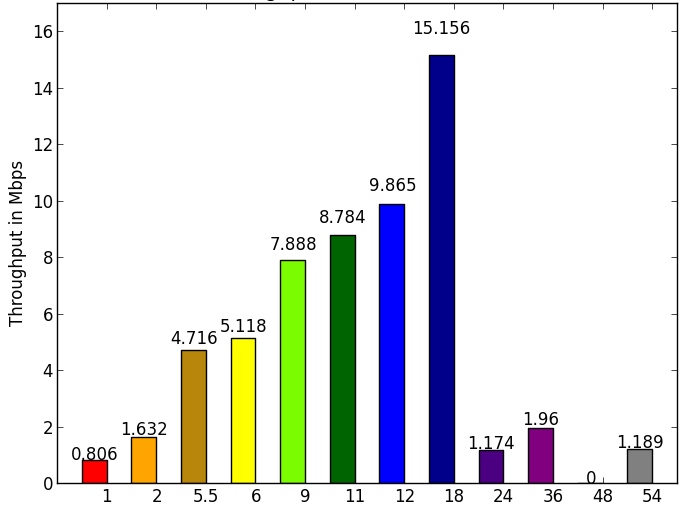
\includegraphics[width=3.75in]{constant.png}\vspace{-2em}
  \caption{dfg}
\end{figure}

\subsection{Testing framework}

Harness.py, etc.

\section{Analysis}

Minstrel actually is better than SampleRate (except on short traces). Eit.

\subsection{Improvements to Minstrel}
Minproved.

\subsection{Availability}
We should make our github repo or something like that available here.

\section{Future Work}

802.11n, SampleRate with EWMA, take data using broadcast approach,  submitting minstrel changes as kernel patch?

\section{Conclusion}

The end.

\section{Acknowledgements}
Jonathan Perry, Hari Balikrishnan, and Derek Smithies. 


{\footnotesize \bibliographystyle{acm}
\bibliography{paper}}

\end{document}






